\chapter{强连通性}

\index{strongly connected graph}

在有向图中，每条边只能沿一个方向通过，因此，即使图是连通的，也不能保证从一个节点到另一个节点一定存在路径。为此，有必要定义一个比连通性要求更强的新概念。

如果从图中任意节点出发都能到达所有其他节点，则称该图是\key{强连通的}。例如，下图左侧的图是强连通图，而右侧的图不是。

\begin{center}
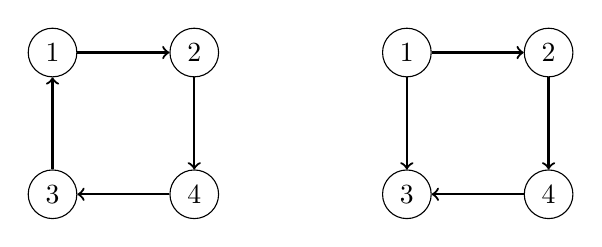
\begin{tikzpicture}[scale=0.9]
\node[draw, circle] (1) at (1,1) {$1$};
\node[draw, circle] (2) at (3,1) {$2$};
\node[draw, circle] (3) at (1,-1) {$3$};
\node[draw, circle] (4) at (3,-1) {$4$};

\path[draw,thick,->] (1) -- (2);
\path[draw,thick,->] (2) -- (4);
\path[draw,thick,->] (4) -- (3);
\path[draw,thick,->] (3) -- (1);

\node[draw, circle] (1b) at (6,1) {$1$};
\node[draw, circle] (2b) at (8,1) {$2$};
\node[draw, circle] (3b) at (6,-1) {$3$};
\node[draw, circle] (4b) at (8,-1) {$4$};

\path[draw,thick,->] (1b) -- (2b);
\path[draw,thick,->] (2b) -- (4b);
\path[draw,thick,->] (4b) -- (3b);
\path[draw,thick,->] (1b) -- (3b);
\end{tikzpicture}
\end{center}

右图不是强连通图，因为例如不存在从节点 2 到节点 1 的路径。

\index{strongly connected component}
\index{component graph}

图的\key{强连通分量}将图划分为尽可能大的强连通部分。所有强连通分量形成一个无环的\key{分量图}，它反映了原图的深层结构。

例如，对于图
\begin{center}
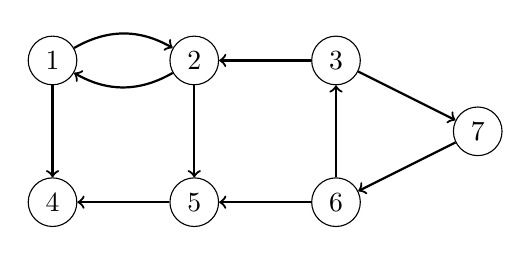
\begin{tikzpicture}[scale=0.9,label distance=-2mm]
\node[draw, circle] (1) at (-1,1) {$7$};
\node[draw, circle] (2) at (-3,2) {$3$};
\node[draw, circle] (4) at (-5,2) {$2$};
\node[draw, circle] (6) at (-7,2) {$1$};
\node[draw, circle] (3) at (-3,0) {$6$};
\node[draw, circle] (5) at (-5,0) {$5$};
\node[draw, circle] (7) at (-7,0) {$4$};

\path[draw,thick,->] (2) -- (1);
\path[draw,thick,->] (1) -- (3);
\path[draw,thick,->] (3) -- (2);
\path[draw,thick,->] (2) -- (4);
\path[draw,thick,->] (3) -- (5);
\path[draw,thick,->] (4) edge [bend left] (6);
\path[draw,thick,->] (6) edge [bend left] (4);
\path[draw,thick,->] (4) -- (5);
\path[draw,thick,->] (5) -- (7);
\path[draw,thick,->] (6) -- (7);
\end{tikzpicture}
\end{center}
其强连通分量如下：
\begin{center}
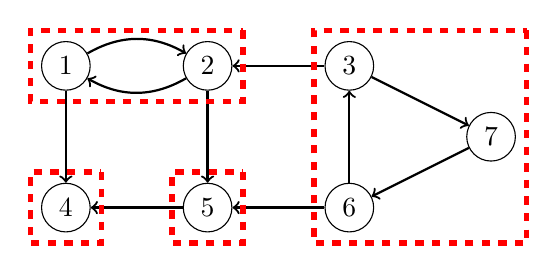
\begin{tikzpicture}[scale=0.9]
\node[draw, circle] (1) at (-1,1) {$7$};
\node[draw, circle] (2) at (-3,2) {$3$};
\node[draw, circle] (4) at (-5,2) {$2$};
\node[draw, circle] (6) at (-7,2) {$1$};
\node[draw, circle] (3) at (-3,0) {$6$};
\node[draw, circle] (5) at (-5,0) {$5$};
\node[draw, circle] (7) at (-7,0) {$4$};

\path[draw,thick,->] (2) -- (1);
\path[draw,thick,->] (1) -- (3);
\path[draw,thick,->] (3) -- (2);
\path[draw,thick,->] (2) -- (4);
\path[draw,thick,->] (3) -- (5);
\path[draw,thick,->] (4) edge [bend left] (6);
\path[draw,thick,->] (6) edge [bend left] (4);
\path[draw,thick,->] (4) -- (5);
\path[draw,thick,->] (5) -- (7);
\path[draw,thick,->] (6) -- (7);

\draw [red,thick,dashed,line width=2pt] (-0.5,2.5) rectangle (-3.5,-0.5);
\draw [red,thick,dashed,line width=2pt] (-4.5,2.5) rectangle (-7.5,1.5);
\draw [red,thick,dashed,line width=2pt] (-4.5,0.5) rectangle (-5.5,-0.5);
\draw [red,thick,dashed,line width=2pt] (-6.5,0.5) rectangle (-7.5,-0.5);
\end{tikzpicture}
\end{center}
对应的分量图如下：
\begin{center}
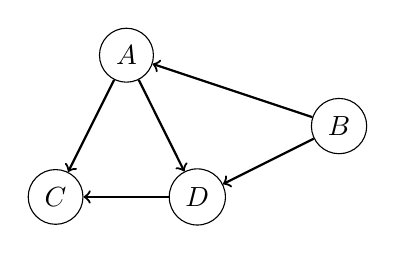
\begin{tikzpicture}[scale=0.9]
\node[draw, circle] (1) at (-3,1) {$B$};
\node[draw, circle] (2) at (-6,2) {$A$};
\node[draw, circle] (3) at (-5,0) {$D$};
\node[draw, circle] (4) at (-7,0) {$C$};

\path[draw,thick,->] (1) -- (2);
\path[draw,thick,->] (1) -- (3);
\path[draw,thick,->] (2) -- (3);
\path[draw,thick,->] (2) -- (4);
\path[draw,thick,->] (3) -- (4);
\end{tikzpicture}
\end{center}
各分量为 $A=\{1,2\}$、$B=\{3,6,7\}$、$C=\{4\}$ 和 $D=\{5\}$。

分量图是无环有向图，因此比原图更容易处理。由于图中不含环，我们总能构造拓扑序，并使用第 16 章介绍的动态规划方法。

\section{Kosaraju 算法}

\index{Kosaraju's algorithm}

\key{Kosaraju 算法}\footnote{据 \cite{aho83} 记载，S. R. Kosaraju 于 1978 年发明了这一算法，但没有发表。1981 年，M. Sharir 再次发现并发表了同一算法 \cite{sha81}。}是一种寻找有向图强连通分量的高效方法。算法执行两次深度优先搜索：第一次搜索根据图的结构构造节点列表，第二次搜索形成强连通分量。

\subsubsection{搜索 1}

Kosaraju 算法的第一阶段按照深度优先搜索处理节点的顺序构造一个列表。算法依次考察所有节点，并从每个尚未处理的节点开始一次深度优先搜索。每个节点在处理完毕后加入列表。

在示例图中，节点的处理顺序如下：
\begin{center}
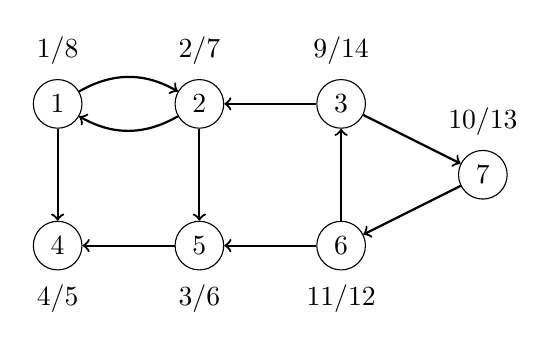
\begin{tikzpicture}[scale=0.9,label distance=-2mm]
\node[draw, circle] (1) at (-1,1) {$7$};
\node[draw, circle] (2) at (-3,2) {$3$};
\node[draw, circle] (4) at (-5,2) {$2$};
\node[draw, circle] (6) at (-7,2) {$1$};
\node[draw, circle] (3) at (-3,0) {$6$};
\node[draw, circle] (5) at (-5,0) {$5$};
\node[draw, circle] (7) at (-7,0) {$4$};

\node at (-7,2.75) {$1/8$};
\node at (-5,2.75) {$2/7$};
\node at (-3,2.75) {$9/14$};
\node at (-7,-0.75) {$4/5$};
\node at (-5,-0.75) {$3/6$};
\node at (-3,-0.75) {$11/12$};
\node at (-1,1.75) {$10/13$};

\path[draw,thick,->] (2) -- (1);
\path[draw,thick,->] (1) -- (3);
\path[draw,thick,->] (3) -- (2);
\path[draw,thick,->] (2) -- (4);
\path[draw,thick,->] (3) -- (5);
\path[draw,thick,->] (4) edge [bend left] (6);
\path[draw,thick,->] (6) edge [bend left] (4);
\path[draw,thick,->] (4) -- (5);
\path[draw,thick,->] (5) -- (7);
\path[draw,thick,->] (6) -- (7);
\end{tikzpicture}
\end{center}

记号 $x/y$ 表示节点在时刻 $x$ 开始处理，在时刻 $y$ 处理完毕。因此，对应的列表如下：

\begin{tabular}{ll}
\\
节点 & 完成时刻 \\
\hline
4 & 5 \\
5 & 6 \\
2 & 7 \\
1 & 8 \\
6 & 12 \\
7 & 13 \\
3 & 14 \\
\\
\end{tabular}
% 
% In the second phase of the algorithm,
% the nodes will be processed
% in reverse order: $[3,7,6,1,2,5,4]$.

\subsubsection{搜索 2}

算法的第二阶段形成图的强连通分量。首先，算法把图中的每条边反向。这保证在第二次搜索中，我们找到的强连通分量不会混入额外节点。

所有边反向后，示例图如下：
\begin{center}
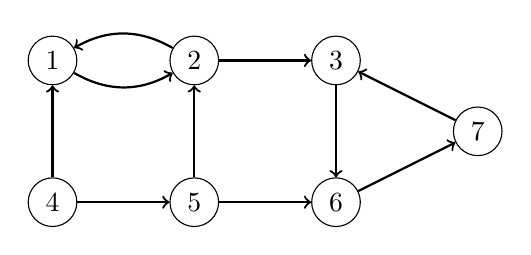
\begin{tikzpicture}[scale=0.9,label distance=-2mm]
\node[draw, circle] (1) at (-1,1) {$7$};
\node[draw, circle] (2) at (-3,2) {$3$};
\node[draw, circle] (4) at (-5,2) {$2$};
\node[draw, circle] (6) at (-7,2) {$1$};
\node[draw, circle] (3) at (-3,0) {$6$};
\node[draw, circle] (5) at (-5,0) {$5$};
\node[draw, circle] (7) at (-7,0) {$4$};

\path[draw,thick,<-] (2) -- (1);
\path[draw,thick,<-] (1) -- (3);
\path[draw,thick,<-] (3) -- (2);
\path[draw,thick,<-] (2) -- (4);
\path[draw,thick,<-] (3) -- (5);
\path[draw,thick,<-] (4) edge [bend left] (6);
\path[draw,thick,<-] (6) edge [bend left] (4);
\path[draw,thick,<-] (4) -- (5);
\path[draw,thick,<-] (5) -- (7);
\path[draw,thick,<-] (6) -- (7);
\end{tikzpicture}
\end{center}

随后，算法按照第一次搜索所得节点列表的\emph{逆序}处理节点。若某节点尚不属于任何分量，算法就创建一个新分量，并从该节点开始深度优先搜索，把搜索发现的所有新节点加入这个分量。

在示例图中，第一个分量从节点 3 开始：

\begin{center}
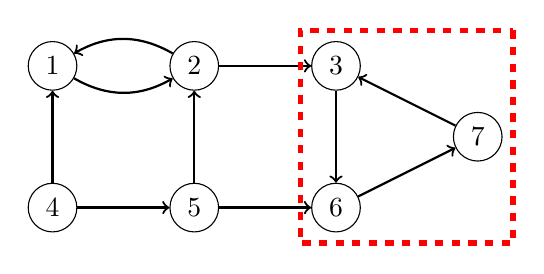
\begin{tikzpicture}[scale=0.9,label distance=-2mm]
\node[draw, circle] (1) at (-1,1) {$7$};
\node[draw, circle] (2) at (-3,2) {$3$};
\node[draw, circle] (4) at (-5,2) {$2$};
\node[draw, circle] (6) at (-7,2) {$1$};
\node[draw, circle] (3) at (-3,0) {$6$};
\node[draw, circle] (5) at (-5,0) {$5$};
\node[draw, circle] (7) at (-7,0) {$4$};

\path[draw,thick,<-] (2) -- (1);
\path[draw,thick,<-] (1) -- (3);
\path[draw,thick,<-] (3) -- (2);
\path[draw,thick,<-] (2) -- (4);
\path[draw,thick,<-] (3) -- (5);
\path[draw,thick,<-] (4) edge [bend left] (6);
\path[draw,thick,<-] (6) edge [bend left] (4);
\path[draw,thick,<-] (4) -- (5);
\path[draw,thick,<-] (5) -- (7);
\path[draw,thick,<-] (6) -- (7);

\draw [red,thick,dashed,line width=2pt] (-0.5,2.5) rectangle (-3.5,-0.5);
\end{tikzpicture}
\end{center}

注意，由于所有边都已反向，这个分量不会“泄漏”到图的其他部分。

\begin{samepage}
列表中的下两个节点是 7 和 6，但它们已经属于某个分量，因此下一个新分量从节点 1 开始：

\begin{center}
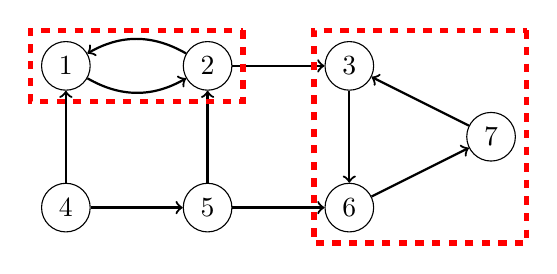
\begin{tikzpicture}[scale=0.9,label distance=-2mm]
\node[draw, circle] (1) at (-1,1) {$7$};
\node[draw, circle] (2) at (-3,2) {$3$};
\node[draw, circle] (4) at (-5,2) {$2$};
\node[draw, circle] (6) at (-7,2) {$1$};
\node[draw, circle] (3) at (-3,0) {$6$};
\node[draw, circle] (5) at (-5,0) {$5$};
\node[draw, circle] (7) at (-7,0) {$4$};

\path[draw,thick,<-] (2) -- (1);
\path[draw,thick,<-] (1) -- (3);
\path[draw,thick,<-] (3) -- (2);
\path[draw,thick,<-] (2) -- (4);
\path[draw,thick,<-] (3) -- (5);
\path[draw,thick,<-] (4) edge [bend left] (6);
\path[draw,thick,<-] (6) edge [bend left] (4);
\path[draw,thick,<-] (4) -- (5);
\path[draw,thick,<-] (5) -- (7);
\path[draw,thick,<-] (6) -- (7);

\draw [red,thick,dashed,line width=2pt] (-0.5,2.5) rectangle (-3.5,-0.5);
\draw [red,thick,dashed,line width=2pt] (-4.5,2.5) rectangle (-7.5,1.5);
%\draw [red,thick,dashed,line width=2pt] (-4.5,0.5) rectangle (-5.5,-0.5);
%\draw [red,thick,dashed,line width=2pt] (-6.5,0.5) rectangle (-7.5,-0.5);
\end{tikzpicture}
\end{center}
\end{samepage}

\begin{samepage}
最后，算法处理节点 5 和 4，建立余下的强连通分量：

\begin{center}
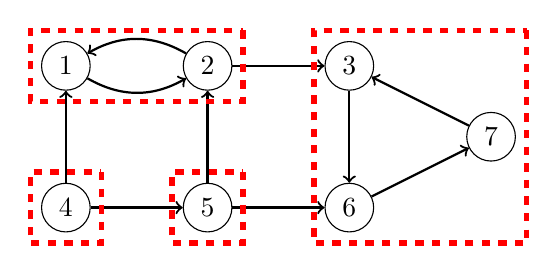
\begin{tikzpicture}[scale=0.9,label distance=-2mm]
\node[draw, circle] (1) at (-1,1) {$7$};
\node[draw, circle] (2) at (-3,2) {$3$};
\node[draw, circle] (4) at (-5,2) {$2$};
\node[draw, circle] (6) at (-7,2) {$1$};
\node[draw, circle] (3) at (-3,0) {$6$};
\node[draw, circle] (5) at (-5,0) {$5$};
\node[draw, circle] (7) at (-7,0) {$4$};

\path[draw,thick,<-] (2) -- (1);
\path[draw,thick,<-] (1) -- (3);
\path[draw,thick,<-] (3) -- (2);
\path[draw,thick,<-] (2) -- (4);
\path[draw,thick,<-] (3) -- (5);
\path[draw,thick,<-] (4) edge [bend left] (6);
\path[draw,thick,<-] (6) edge [bend left] (4);
\path[draw,thick,<-] (4) -- (5);
\path[draw,thick,<-] (5) -- (7);
\path[draw,thick,<-] (6) -- (7);

\draw [red,thick,dashed,line width=2pt] (-0.5,2.5) rectangle (-3.5,-0.5);
\draw [red,thick,dashed,line width=2pt] (-4.5,2.5) rectangle (-7.5,1.5);
\draw [red,thick,dashed,line width=2pt] (-4.5,0.5) rectangle (-5.5,-0.5);
\draw [red,thick,dashed,line width=2pt] (-6.5,0.5) rectangle (-7.5,-0.5);
\end{tikzpicture}
\end{center}
\end{samepage}

算法执行两次深度优先搜索，因此时间复杂度为 $O(n+m)$。

\section{2SAT 问题}

\index{2SAT problem}

强连通性还与\key{2SAT 问题}\footnote{这里介绍的算法最初见于 \cite{asp79}。另有一种著名的线性时间算法 \cite{eve75}，它基于回溯。}有关。在这个问题中，给定逻辑公式
\[
(a_1 \lor b_1) \land (a_2 \lor b_2) \land \cdots \land (a_m \lor b_m),
\]
其中每个 $a_i$ 和 $b_i$ 要么是逻辑变量（$x_1,x_2,\ldots,x_n$），要么是逻辑变量的否定（$\lnot x_1, \lnot x_2, \ldots, \lnot x_n$）。符号“$\land$”和“$\lor$”分别表示逻辑运算“与”和“或”。我们的任务是为每个变量赋值，使公式为真；或者说明无法做到。

例如，公式
\[
L_1 = (x_2 \lor \lnot x_1) \land
      (\lnot x_1 \lor \lnot x_2) \land
      (x_1 \lor x_3) \land
      (\lnot x_2 \lor \lnot x_3) \land
      (x_1 \lor x_4)
\]
在变量取值如下时为真：

\[
\begin{cases}
x_1 = \textrm{false} \\
x_2 = \textrm{false} \\
x_3 = \textrm{true} \\
x_4 = \textrm{true} \\
\end{cases}
\]

然而，无论如何赋值，公式
\[
L_2 = (x_1 \lor x_2) \land
      (x_1 \lor \lnot x_2) \land
      (\lnot x_1 \lor x_3) \land
      (\lnot x_1 \lor \lnot x_3)
\]
都为假。这是因为给 $x_1$ 选择任何值都会产生矛盾。若 $x_1$ 为假，则 $x_2$ 和 $\lnot x_2$ 必须同时为真，这是不可能的；若 $x_1$ 为真，则 $x_3$ 和 $\lnot x_3$ 必须同时为真，同样不可能。

2SAT 问题可以表示为一个图，其中节点对应变量 $x_i$ 及其否定 $\lnot x_i$，边表示变量之间的蕴含关系。每个子句 $(a_i \lor b_i)$ 生成两条边：$\lnot a_i \to b_i$ 和 $\lnot b_i \to a_i$。这表示若 $a_i$ 不成立，则 $b_i$ 必须成立，反之亦然。

公式 $L_1$ 对应的图为：
\\
\begin{center}
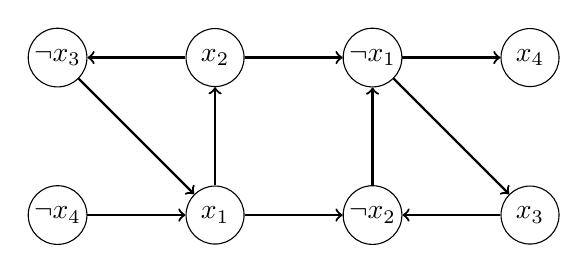
\begin{tikzpicture}[scale=1.0,minimum size=2pt]
\node[draw, circle, inner sep=1.3pt] (1) at (1,2) {$\lnot x_3$};
\node[draw, circle] (2) at (3,2) {$x_2$};
\node[draw, circle, inner sep=1.3pt] (3) at (1,0) {$\lnot x_4$};
\node[draw, circle] (4) at (3,0) {$x_1$};
\node[draw, circle, inner sep=1.3pt] (5) at (5,2) {$\lnot x_1$};
\node[draw, circle] (6) at (7,2) {$x_4$};
\node[draw, circle, inner sep=1.3pt] (7) at (5,0) {$\lnot x_2$};
\node[draw, circle] (8) at (7,0) {$x_3$};
 
\path[draw,thick,->] (1) -- (4);
\path[draw,thick,->] (4) -- (2);
\path[draw,thick,->] (2) -- (1);
\path[draw,thick,->] (3) -- (4);
\path[draw,thick,->] (2) -- (5);
\path[draw,thick,->] (4) -- (7);
\path[draw,thick,->] (5) -- (6);
\path[draw,thick,->] (5) -- (8);
\path[draw,thick,->] (8) -- (7);
\path[draw,thick,->] (7) -- (5);
\end{tikzpicture}
\end{center}
公式 $L_2$ 对应的图为：
\\
\begin{center}
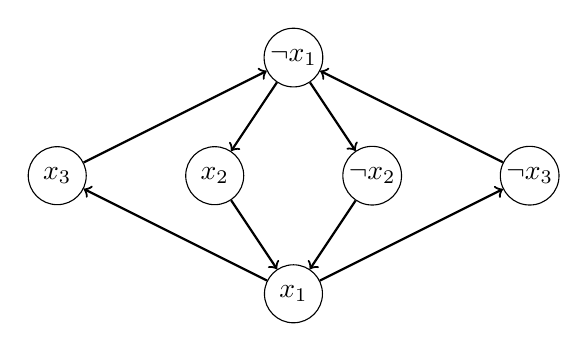
\begin{tikzpicture}[scale=1.0,minimum size=2pt]
\node[draw, circle] (1) at (1,2) {$x_3$};
\node[draw, circle] (2) at (3,2) {$x_2$};
\node[draw, circle, inner sep=1.3pt] (3) at (5,2) {$\lnot x_2$};
\node[draw, circle, inner sep=1.3pt] (4) at (7,2) {$\lnot x_3$};
\node[draw, circle, inner sep=1.3pt] (5) at (4,3.5) {$\lnot x_1$};
\node[draw, circle] (6) at (4,0.5) {$x_1$};

\path[draw,thick,->] (1) -- (5);
\path[draw,thick,->] (4) -- (5);
\path[draw,thick,->] (6) -- (1);
\path[draw,thick,->] (6) -- (4);
\path[draw,thick,->] (5) -- (2);
\path[draw,thick,->] (5) -- (3);
\path[draw,thick,->] (2) -- (6);
\path[draw,thick,->] (3) -- (6);
\end{tikzpicture}
\end{center}

图的结构告诉我们是否能够为变量赋值，使公式为真。事实证明，当且仅当不存在某个 $i$，使节点 $x_i$ 与 $\lnot x_i$ 同属一个强连通分量时，才存在这样的赋值。如果存在这类节点，图中既有从 $x_i$ 到 $\lnot x_i$ 的路径，也有从 $\lnot x_i$ 到 $x_i$ 的路径，因此 $x_i$ 和 $\lnot x_i$ 都必须为真，这是不可能的。

公式 $L_1$ 的图中不存在同属一个强连通分量的 $x_i$ 和 $\lnot x_i$，因此存在解。公式 $L_2$ 的图中所有节点都属于同一个强连通分量，因此无解。

若解存在，可以按照逆拓扑序遍历分量图中的节点来确定变量值。每一步处理一个不存在指向未处理分量的边的分量。如果分量中的变量尚未赋值，就根据该分量内的文字确定它们的值；若已经赋值，则保持不变。重复此过程，直到每个变量都得到一个值。

公式 $L_1$ 的分量图如下：
\begin{center}
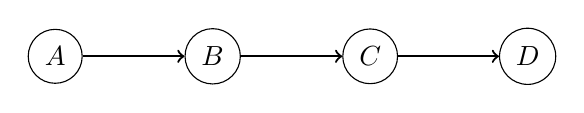
\begin{tikzpicture}[scale=1.0]
\node[draw, circle] (1) at (0,0) {$A$};
\node[draw, circle] (2) at (2,0) {$B$};
\node[draw, circle] (3) at (4,0) {$C$};
\node[draw, circle] (4) at (6,0) {$D$};

\path[draw,thick,->] (1) -- (2);
\path[draw,thick,->] (2) -- (3);
\path[draw,thick,->] (3) -- (4);
\end{tikzpicture}
\end{center}

各分量为 $A = \{\lnot x_4\}$、$B = \{x_1, x_2, \lnot x_3\}$、$C = \{\lnot x_1, \lnot x_2, x_3\}$ 和 $D = \{x_4\}$。构造解时，先处理分量 $D$，令 $x_4$ 为真；随后处理分量 $C$，令 $x_1$ 和 $x_2$ 为假，$x_3$ 为真。所有变量都已赋值，因此余下的分量 $A$ 和 $B$ 不再改变变量值。

这种方法能够成立，是因为该图具有特殊结构：若存在从节点 $x_i$ 到节点 $x_j$ 的路径，以及从节点 $x_j$ 到节点 $\lnot x_j$ 的路径，那么节点 $x_i$ 永远不会取真。原因是，此时也存在从节点 $\lnot x_j$ 到节点 $\lnot x_i$ 的路径，于是 $x_i$ 和 $x_j$ 都取假。

\index{3SAT problem}

更困难的是\key{3SAT 问题}，其中公式的每个部分都形如 $(a_i \lor b_i \lor c_i)$。该问题是 NP 困难的，目前没有已知的高效算法。
